\documentclass[10pt,openany,a4paper]{article}
\usepackage{graphicx} 
\usepackage{multirow}
\usepackage{enumitem}
\usepackage{amssymb}
\usepackage{amsmath}
\usepackage{xcolor}
\usepackage{cancel}
\usepackage{tcolorbox}
\usepackage{geometry}
\usepackage{tikz}
	\geometry{
		total = {160mm, 237mm},
		left = 25mm,
		right = 35mm,
		top = 30mm,
		bottom = 30mm,
	}

\begin{document}
    \pagenumbering{gobble}
    \begin{tabular}{|lcl|}
     \hline
     Nama&:&Teosofi Hidayah Agung\\
     NRP&:&5002221132\\
     \hline
    \end{tabular}

    \begin{enumerate}
        \begin{tcolorbox}[title=Deret Fourier, colback=lightgray]
            $f(x)$ fungsi periodik pada interval $-L\leq x\leq L$ dimana $f(x+2L)=f(x)$.
            Sehingga $f(x)$ dapat ditulis sebagai berikut
            \[f(x)=\frac{a_0}{2}+\sum_{n=1}^{\infty}\left[a_n\cos\left(\frac{n\pi x}{L}\right)+b_n\sin\left(\frac{n\pi x}{L}\right)\right]\]
            dimana
            \begin{align}
                a_0&=\frac{1}{L}\int_{-L}^{L}f(x)\,dx\\
                a_n&=\frac{1}{L}\int_{-L}^{L}f(x)\cos\left(\frac{n\pi x}{L}\right)\,dx\\
                b_n&=\frac{1}{L}\int_{-L}^{L}f(x)\sin\left(\frac{n\pi x}{L}\right)\,dx
            \end{align}
        \end{tcolorbox}

        \item[1(g).] $f(x)=\begin{cases}
            0,&\quad -\pi\leq x\leq 0\\
            x^2,&\quad 0<x\leq\pi
        \end{cases},\,f(x+2\pi)=f(x)$\\
        \textbf{Jawab}:
        \begin{flalign*}
            a_0&=\frac{1}{\pi}\int_{-\pi}^{\pi}f(x)\,dx&\\
            &=\frac{1}{\pi}\left[\int_{-\pi}^{0}f(x)\,dx+\int_{0}^{\pi}f(x)\,dx\right]&\\
            &=\frac{1}{\pi}\left[0+\int_{0}^{\pi}x^2\,dx\right]&\\
            &=\frac{1}{\pi}\left[\frac{1}{3}x^3\right]_{0}^{\pi}=\frac{\pi^2}{3}
        \end{flalign*}
        \begin{flalign*}
            a_n&=\frac{1}{\pi}\int_{-\pi}^{\pi}f(x)\cos\left(\frac{n\cancel{\pi} x}{\cancel{\pi}}\right)\,dx&\\
            &=\frac{1}{\pi}\left[\int_{-\pi}^{0}f(x)\cos\left(nx\right)\,dx+\int_{0}^{\pi}f(x)\cos\left(nx\right)\,dx\right]&\\
            &=\frac{1}{\pi}\left[0+\int_{0}^{\pi}x^2\cos\left(nx\right)\,dx\right]&\\
            &=\frac{1}{\pi}\left[\frac{x^2}{n}\sin(nx)+\frac{2x}{n^2}\cos(nx)-\frac{2}{n^3}\sin(nx)\right]_{0}^{\pi}&\\
            &=\frac{1}{n^3\pi}\left[\underbrace{n^2x^2\sin(nx)}_{0}+2nx\cos(nx)-\underbrace{2\sin(nx)}_0\right]_{0}^{\pi}&\\
            &=\frac{1}{n^3\pi}\left[2n\pi\cos(n\pi)-0\right]&\\
            &=\frac{2}{n^2}\cos(n\pi)=\begin{cases}
                -&\frac{2}{n^2},\quad n \textrm{ ganjil}\\
                &\frac{2}{n^2},\quad n \textrm{ genap}
            \end{cases}&\\
        \end{flalign*}
        \begin{flalign*}
            b_n&=\frac{1}{\pi}\int_{-\pi}^{\pi}f(x)\sin\left(\frac{n\cancel{\pi} x}{\cancel{\pi}}\right)\,dx&\\
            &=\frac{1}{\pi}\left[\int_{-\pi}^{0}f(x)\sin\left(nx\right)\,dx+\int_{0}^{\pi}f(x)\sin\left(nx\right)\,dx\right]&\\
            &=\frac{1}{\pi}\left[0+\int_{0}^{\pi}x^2\sin\left(nx\right)\,dx\right]&\\
            &=\frac{1}{\pi}\left[-\frac{x^2}{n}\cos(nx)+\frac{2x}{n^2}\sin(nx)+\frac{2}{n^3}\cos(nx)\right]_{0}^{\pi}&\\
            &=\frac{1}{n^3\pi}\left[-n^2x^2\cos(nx)+\underbrace{2nx\sin(nx)}_0+2\cos(nx)\right]_{0}^{\pi}&\\
            &=\frac{1}{n^3\pi}\left[-n^2{\pi}^2\cos(n\pi)+0+2\cos(n\pi)-(-0+0+2)\right]&\\
            &=\frac{1}{n^3\pi}\left[-n^2{\pi}^2\cos(n\pi)+2\cos(n\pi)-2\right]&\\
            &=\begin{cases}
                &\frac{\pi}{n}-\frac{4}{n^3\pi},\quad n \textrm{ ganjil}\\
                &\frac{\pi}{n},\quad n \textrm{ genap}
            \end{cases}
        \end{flalign*}
        Sehingga deret fourier-nya adalah
        \begin{flalign*}
            f(x)=\frac{\pi^2}{6}&+\sum_{n=1}^{\infty}\left[-\frac{2}{(2n-1)^2}\cos((2n-1)x)+\left(\frac{\pi}{2n-1}-\frac{4}{(2n-1)^3\pi}\right)\sin((2n-1)x)\right]&\\
            &+\sum_{m=1}^{\infty}\left[\frac{1}{2m^2}\cos(2mx)+\frac{\pi}{2m}\sin(2mx)\right]
        \end{flalign*}\\
        
        \item[1(l).] $f(x)=\begin{cases}
            2-x,&\quad 0\leq x\leq 4\\
            x-6,&\quad 4<x\leq 8
        \end{cases},\,f(x+8)=f(x)$\\
        \textbf{Jawab}:
        \begin{flalign*}
            a_0&=\frac{1}{4}\int_{0}^{8}f(x)\,dx&\\
            &=\frac{1}{4}\left[\int_{0}^{4}f(x)\,dx+\int_{4}^{8}f(x)\,dx\right]&\\
            &=\frac{1}{4}\left[\int_{0}^{4}2-x\,dx+\int_{4}^{8}x-6\,dx\right]&\\
            &=\frac{1}{4}\left[\left.2x-\frac{1}{2}x^2\right|_{0}^{4}+\left.\frac{1}{2}x^2-6x\right|_{4}^{8}\right]&\\
            &=\frac{1}{4}\left[(8-8-0)+(-16+16)\right]=0
        \end{flalign*}
        \begin{flalign*}
            a_n&=\frac{1}{4}\int_{0}^{8}f(x)\cos\left(\frac{n\pi x}{4}\right)\,dx&\\
            &=\frac{1}{4}\left[\int_{0}^{4}(2-x)\cos\left(\frac{n\pi x}{4}\right)\,dx+\int_{4}^{8}(x-6)\cos\left(\frac{n\pi x}{4}\right)\,dx\right]&\\
            &=\frac{1}{4}\left[\underbrace{\int_{0}^{4}2\cos\left(\frac{n\pi x}{4}\right)\,dx}_0-\int_{0}^{4}x\cos\left(\frac{n\pi x}{4}\right)\,dx+\int_{4}^{8}x\cos\left(\frac{n\pi x}{4}\right)\,dx-\underbrace{\int_{4}^{8}6\cos\left(\frac{n\pi x}{4}\right)\,dx}_0\right]&\\
            &=\frac{1}{4}\left[\int_{4}^{8}x\cos\left(\frac{n\pi x}{4}\right)\,dx-\int_{0}^{4}x\cos\left(\frac{n\pi x}{4}\right)\,dx\right]&\\
            &=\frac{1}{4}\left[\left.\underbrace{\frac{4x}{n\pi}\sin\left(\frac{n\pi x}{4}\right)}_0+\frac{16}{n^2\pi^2}\cos\left(\frac{n\pi x}{4}\right)\right|_{4}^{8}+\left.\underbrace{\frac{4x}{n\pi}\sin\left(\frac{n\pi x}{4}\right)}_0+\frac{16}{n^2\pi^2}\cos\left(\frac{n\pi x}{4}\right)\right|_{4}^{0}\right]&\\
            &=\frac{1}{4}\left[\left.\frac{16}{n^2\pi^2}\cos\left(\frac{n\pi x}{4}\right)\right|_{4}^{8}+\left.\frac{16}{n^2\pi^2}\cos\left(\frac{n\pi x}{4}\right)\right|_{4}^{0}\right]&\\
            &=\frac{4}{n^2\pi^2}\left[\left.\cos\left(\frac{n\pi x}{4}\right)\right|_{4}^{8}+\left.\cos\left(\frac{n\pi x}{4}\right)\right|_{4}^{0}\right]&\\
            &=\frac{4}{n^2\pi^2}\left[\underbrace{\cos\left(2n\pi\right)}_1-\cos\left(n\pi\right)+\cos\left(0\right)-\cos\left(n\pi\right)\right]&\\
            &=\frac{4}{n^2\pi^2}\left[2-2\cos\left(n\pi\right)\right]=\begin{cases}
                \frac{16}{n^2\pi^2}&, \quad n \textrm{ ganjil}\\
                0&,\quad n \textrm{ genap}
            \end{cases}&\\
        \end{flalign*}
        \begin{flalign*}
            b_n&=\frac{1}{4}\int_{0}^{8}f(x)\sin\left(\frac{n\pi x}{4}\right)\,dx&\\
            &=\frac{1}{4}\left[\int_{0}^{4}(2-x)\sin\left(\frac{n\pi x}{4}\right)\,dx+\int_{4}^{8}(x-6)\sin\left(\frac{n\pi x}{4}\right)\,dx\right]&\\
            &=\frac{1}{4}\left[\int_{0}^{4}2\sin\left(\frac{n\pi x}{4}\right)\,dx-\int_{0}^{4}x\sin\left(\frac{n\pi x}{4}\right)\,dx+\int_{4}^{8}x\sin\left(\frac{n\pi x}{4}\right)\,dx-\int_{4}^{8}6\sin\left(\frac{n\pi x}{4}\right)\,dx\right]&\\
            &=\frac{1}{4}\left[\left.-\frac{8}{n\pi}\cos\left(\frac{n\pi x}{4}\right)\right|_{0}^{4}+\left.\frac{24}{n\pi}\cos\left(\frac{n\pi x}{4}\right)\right|_{4}^{8}-\int_{0}^{4}x\sin\left(\frac{n\pi x}{4}\right)\,dx+\int_{4}^{8}x\sin\left(\frac{n\pi x}{4}\right)\,dx\right]&\\
            &=\frac{1}{4}\left[\frac{16}{n\pi}+\frac{48}{n\pi}-\int_{0}^{4}x\sin\left(\frac{n\pi x}{4}\right)\,dx+\int_{4}^{8}x\sin\left(\frac{n\pi x}{4}\right)\,dx\right]&\\
            &=\frac{1}{4}\left[\frac{64}{n\pi}-\left(\left.-\frac{4x}{n\pi}\cos\left(\frac{n\pi x}{4}\right)+\underbrace{\frac{16}{n^2\pi^2}\sin\left(\frac{n\pi x}{4}\right)}_0\right|_{0}^{4}\right)-\left.\frac{4x}{n\pi}\cos\left(\frac{n\pi x}{4}\right)+\underbrace{\frac{16}{n^2\pi^2}\sin\left(\frac{n\pi x}{4}\right)}_0\right|_{4}^{8}\right]&\\
            &=\frac{1}{4}\left[\frac{64}{n\pi}+\left.\frac{4x}{n\pi}\cos\left(\frac{n\pi x}{4}\right)\right|_{0}^{4}-\left.\frac{4x}{n\pi}\cos\left(\frac{n\pi x}{4}\right)\right|_{4}^{8}\right]&\\
            &=\frac{1}{4}\left[\frac{64}{n\pi}+\frac{16}{n\pi}\cos(n\pi)-0-\frac{32}{n\pi}+\frac{16}{n\pi}\cos(n\pi)\right]&\\
            &=\frac{1}{4}\left[\frac{32}{n\pi}+\frac{32}{n\pi}\cos(n\pi)\right]&\\
            &=\frac{8}{n\pi}+\frac{8}{n\pi}\cos(n\pi)=\begin{cases}
                0&, \quad n \textrm{ ganjil}\\
                \frac{16}{n\pi}&,\quad n \textrm{ genap}
            \end{cases}
        \end{flalign*}
        Sehingga deret fourier-nya adalah
        \begin{align*}
            f(x)&=\sum_{n=1}^{\infty}\frac{16}{(2n-1)\pi^2}\cos\left(\frac{(2n-1)\pi x}{4}\right)+\sum_{n=1}^{\infty}\frac{16}{2n\pi}\sin\left(\frac{n\pi x}{2}\right)\\
            &=\frac{16}{\pi^2}\sum_{n=1}^{\infty}\frac{1}{2n-1}\cos\left(\frac{(2n-1)\pi x}{4}\right)+\frac{8}{\pi}\sum_{n=1}^{\infty}\frac{1}{n}\sin\left(\frac{n\pi x}{2}\right)
        \end{align*}\\

        \item[2.] Hasil dari penderetan menurut Fourier $f(x)=\begin{cases}
            0,&\quad -\pi\leq x\leq 0\\
            1,&\quad 0<x\leq\pi
        \end{cases},\,f(x+2\pi)=f(x)$ untuk, $0<x<\pi$ adalah
        \[f(x)=\frac{1}{2}+\frac{2}{\pi}\sum_{n=1}^{\infty}\frac{\sin(2n-1)x}{2n-1}\]
        untuk nilai $x$ berapakah, sehingga dapat ditunjukkan nilai deret berikut ini adalah benar
        \[\frac{\pi}{4}=1-\frac{1}{3}+\frac{1}{5}-\frac{1}{7}+\dots\]
        \textbf{Jawab}:
        \begin{flalign*}
            \boxed{x=\frac{\pi}{2}}\\
            f\left(\frac{\pi}{2}\right)&= \frac{1}{2}+\frac{2}{\pi}\sum_{n=1}^{\infty}\frac{\sin\left(\frac{(2n-1)\pi}{2}\right)}{2n-1}&\\
            1&= \frac{1}{2}+\frac{2}{\pi}\left(\sin\left(\frac{\pi}{2}\right)+\frac{1}{3}\sin\left(\frac{3\pi}{2}\right)+\frac{1}{5}\sin\left(\frac{5\pi}{2}\right)+\dots\right)&\\
            \frac{1}{2}&=\frac{2}{\pi}\left(1-\frac{1}{3}+\frac{1}{5}-\frac{1}{7}+\dots\right)&\\
            \frac{\pi}{4}&=1-\frac{1}{3}+\frac{1}{5}-\frac{1}{7}+\dots\quad\blacksquare
        \end{flalign*}\\

        \item[(+).] $f(x)=\begin{cases}
            \cos x,&\quad 0\leq x\leq \pi\\
            0,&\quad \pi<x\leq 2\pi
        \end{cases},\,f(x+2\pi)=f(x)$\\
        \textbf{Jawab}:
        \begin{flalign*}
            a_0&=\frac{1}{\pi}\int_{0}^{2\pi}f(x)\,dx&\\
            &=\frac{1}{\pi}\left[\int_{0}^{\pi}f(x)\,dx+\int_{\pi}^{2\pi}f(x)\,dx\right]&\\
            &=\frac{1}{\pi}\left[\int_{0}^{\pi}\cos(x)\,dx+0\right]=0&\\
        \end{flalign*}
        \begin{flalign*}
            a_n&=\frac{1}{\pi}\int_{0}^{2\pi}f(x)\cos\left(\frac{n\cancel{\pi} x}{\cancel{\pi}}\right)\,dx&\\
            &=\frac{1}{\pi}\left[\int_{0}^{\pi}f(x)\cos(nx)\,dx+\int_{\pi}^{2\pi}f(x)\cos(nx)\,dx\right]&\\
            &=\frac{1}{\pi}\left[\int_{0}^{\pi}\cos(x)\cos(nx)\,dx+0\right]&\\
            &=\frac{1}{\pi}\int_{0}^{\pi}\cos(x)\cos(nx)\,dx=\begin{cases}
                &\frac{1}{2},\quad n=1\\
                &0,\quad n\textrm{ yang lain}
            \end{cases}&\\
        \end{flalign*}
        \begin{flalign*}
            b_n&=\frac{1}{\pi}\int_{0}^{2\pi}f(x)\sin\left(\frac{n\cancel{\pi} x}{\cancel{\pi}}\right)\,dx&\\
            &=\frac{1}{\pi}\left[\int_{0}^{\pi}f(x)\sin(nx)\,dx+\int_{\pi}^{2\pi}f(x)\sin(nx)\,dx\right]&\\
            &=\frac{1}{\pi}\left[\int_{0}^{\pi}\cos(x)\sin(nx)\,dx+0\right]&\\
            &=\frac{1}{2\pi}\left[\int_{0}^{\pi}\sin(nx+x)+\sin(nx-x)\,dx\right]&\\
            &=\frac{1}{2\pi}\left[\int_{0}^{\pi}\sin((n+1)x)+\sin((n-1)x)\,dx\right]&\\
            &=\frac{1}{2\pi}\left[\frac{-\cos((n+1)x)}{n+1}-\frac{\cos((n-1)x)}{n-1}\right]_{0}^{\pi}&\\
            &=\frac{1}{2\pi}\left[-\frac{\cos((n+1)\pi)}{n+1}-\frac{\cos((n-1)\pi)}{n-1}+\frac{1}{n+1}+\frac{1}{n-1}\right]&\\
            &=\frac{1}{2\pi}\left[-\frac{(n-1)\cos((n+1)\pi)-(n+1)\cos((n-1)\pi)+2n}{n^2-1}\right]&\\
            &=\begin{cases}
                0&, \quad n \textrm{ ganjil}\\
                \frac{2n}{(n^2-1)\pi}&,\quad n \textrm{ genap}
            \end{cases}
        \end{flalign*}
        Sehingga deret fourier-nya adalah
        \begin{align*}
            f(x)&=\frac{1}{2}\cos(x)+\sum_{n=1}^{\infty}\frac{4n}{(4n^2-1)\pi}\sin(2nx)
        \end{align*}\\

        \item[6.] Diberikan fungsi $f(x)=e^{-x}$
        \begin{enumerate}[label=(\alph*)]
            \item Dapatkan deret fourier dari $f(x)$ untuk $-\pi\leq x\leq\pi$.\\
            \textbf{Jawab}:
            \begin{flalign*}
                a_0&=\frac{1}{\pi}\int_{-\pi}^{\pi}f(x)\,dx&\\
                &=\frac{1}{\pi}\int_{-\pi}^{\pi}e^{-x}\,dx&\\
                &=\frac{1}{\pi}\left[-e^{-x}\right]_{-\pi}^{\pi}&\\
                &=\frac{1}{\pi}\left[-e^{-\pi}+e^{\pi}\right]&\\
                &=\frac{1}{\pi}\left[e^{\pi}-e^{-\pi}\right]&\\
            \end{flalign*}
            \begin{flalign*}
                a_n&=\frac{1}{\pi}\int_{-\pi}^{\pi}e^{-x}\cos\left(\frac{n\cancel{\pi} x}{\cancel{\pi}}\right)\,dx&\\
                &=\frac{1}{\pi}\int_{-\pi}^{\pi}e^{-x}\cos\left(nx\right)\,dx&\\
                &=\frac{1}{\pi}\left[\frac{ne^{-x}\sin(nx)-e^{-x}\cos(nx)}{n^2+1}\right]_{-\pi}^{\pi}&\\
                &=\frac{1}{(n^2+1)\pi}\left[ne^{-x}\sin(nx)-e^{-x}\cos(nx)\right]_{-\pi}^{\pi}&\\
                &=\frac{1}{(n^2+1)\pi}\left[ne^{-\pi}\sin(n\pi)-e^{-\pi}\cos(n\pi)-(ne^{\pi}\sin(-n\pi)-e^{\pi}\cos(-n\pi))\right]&\\
                &=\frac{1}{(n^2+1)\pi}\left[0-e^{-\pi}\cos(n\pi)-(0-e^{\pi}\cos(-n\pi))\right]&\\
                &=\frac{1}{(n^2+1)\pi}\left[e^{\pi}\cos(n\pi)-e^{-\pi}\cos(n\pi)\right]&\\
                &=\frac{e^{\pi}-e^{-\pi}}{(n^2+1)\pi}(-1)^n&\\
            \end{flalign*}
            \begin{flalign*}
                b_n&=\frac{1}{\pi}\int_{-\pi}^{\pi}e^{-x}\sin\left(\frac{n\cancel{\pi} x}{\cancel{\pi}}\right)\,dx&\\
                &=\frac{1}{\pi}\int_{-\pi}^{\pi}e^{-x}\sin\left(nx\right)\,dx&\\
                &=\frac{1}{\pi}\left[\frac{-ne^{-x}\cos(nx)-e^{-x}\sin(nx)}{n^2+1}\right]_{-\pi}^{\pi}&\\
                &=\frac{1}{(n^2+1)\pi}\left[-ne^{-x}\cos(nx)-e^{-x}\sin(nx)\right]_{-\pi}^{\pi}&\\
                &=\frac{1}{(n^2+1)\pi}\left[-ne^{-\pi}\cos(n\pi)-e^{-\pi}\sin(n\pi)-(-ne^{\pi}\cos(n-\pi)-e^{\pi}\sin(n-\pi))\right]&\\
                &=\frac{1}{(n^2+1)\pi}\left[-ne^{-\pi}\cos(n\pi)-0-(-ne^{\pi}\cos(-n\pi)-0)\right]&\\
                &=\frac{1}{(n^2+1)\pi}\left[ne^{\pi}\cos(n\pi)-ne^{-\pi}\cos(n\pi)\right]&\\
                &=\frac{e^{\pi}-e^{-\pi}}{(n^2+1)\pi}(-1)^nn&\\
            \end{flalign*}
            $\therefore$ Deret fouriernya adalah
            \[f(x)=\frac{e^{\pi}-e^{-\pi}}{2\pi}+\frac{e^{\pi}-e^{-\pi}}{\pi}\sum_{n=1}^{\infty}\left(\frac{(-1)^n}{n^2+1}\right)\cos(nx)+n\sin(nx)\]
                
            \item Ekspansikan $f(x)$ ke dalam deret cosinus fourier untuk $0 \leq x\leq\pi$.
            \begin{flalign*}
                a_0&=\frac{2}{\pi}\int_{0}^{\pi}e^{-x}\,dx&\\
                &=\frac{2}{\pi}\left[-e^{-x}\right]_{0}^{\pi}&\\
                &=\frac{2}{\pi}\left[-e^{-\pi}+e^{0}\right]&\\
                &=\frac{2(1-e^{-\pi})}{\pi}&\\
            \end{flalign*}
            \begin{flalign*}
                a_n&=\frac{2}{\pi}\int_{0}^{\pi}e^{-x}\cos\left(\frac{n\cancel{\pi} x}{\frac{\cancel{\pi}}{2}}\right)\,dx&\\
                &=\frac{2}{\pi}\int_{0}^{\pi}e^{-x}\cos\left(2nx\right)\,dx&\\
                &=\frac{2}{\pi}\left[\frac{2ne^{-x}\sin(2nx)-e^{-x}\cos(2nx)}{4n^2+1}\right]_{0}^{\pi}&\\
                &=\frac{2}{(4n^2+1)\pi}\left[2ne^{-x}\sin(2nx)-e^{-x}\cos(2nx)\right]_{0}^{\pi}&\\
                &=\frac{2}{(4n^2+1)\pi}\left[2ne^{-\pi}\sin(2n\pi)-e^{-\pi}\cos(2n\pi)-(2ne^{0}\sin(0)-e^{0}\cos(0))\right]&\\
                &=\frac{2}{(4n^2+1)\pi}\left[0-e^{-\pi}\cos(2n\pi)-(0-1)\right]&\\
                &=\frac{2}{(4n^2+1)\pi}\left[1-e^{-\pi}\cos(2n\pi)\right]&\\
                &=\frac{2}{(4n^2+1)\pi}\left[1-e^{-\pi}\right]&\\
                &=\frac{2(1-e^{-\pi})}{(4n^2+1)\pi}&\\
            \end{flalign*}
            $\therefore$ Deret fouriernya adalah
            \[f(x)=\frac{1-e^{-\pi}}{\pi}+\frac{2(1-e^{-\pi})}{\pi}\sum_{n=1}^{\infty}\frac{1}{4n^2+1}\cos(2nx)\]

            \item Ekspansikan $f(x)$ ke dalam deret sinus fourier untuk $0 \leq x<\pi$.
            \begin{flalign*}
                b_n&=\frac{2}{\pi}\int_{0}^{\pi}e^{-x}\sin\left(\frac{n\cancel{\pi} x}{\frac{\cancel{\pi}}{2}}\right)\,dx&\\
                &=\frac{2}{\pi}\int_{0}^{\pi}e^{-x}\sin\left(2nx\right)\,dx&\\
                &=\frac{2}{\pi}\left[\frac{-2ne^{-x}\cos(2nx)-e^{-x}\sin(2nx)}{4n^2+1}\right]_{0}^{\pi}&\\
                &=\frac{2}{(4n^2+1)\pi}\left[-2ne^{-x}\cos(2nx)-e^{-x}\sin(2nx)\right]_{0}^{\pi}&\\
                &=\frac{2}{(4n^2+1)\pi}\left[-2ne^{-\pi}\cos(2n\pi)-e^{-\pi}\sin(2n\pi)-(-2ne^{0}\cos(0)-e^{0}\sin(0))\right]&\\
                &=\frac{2}{(4n^2+1)\pi}\left[-2ne^{-\pi}-0-(-2n-0)\right]&\\
                &=\frac{2}{(4n^2+1)\pi}\left[2n-2ne^{-\pi}\right]&\\
                &=\frac{4n(1-e^{-\pi})}{(4n^2+1)\pi}&\\
            \end{flalign*}
            $\therefore$ Deret fouriernya adalah
            \[f(x)=\frac{4(1-e^{-\pi})}{\pi}\sum_{n=1}^{\infty}\frac{n}{4n^2+1}\sin(2nx)\]

            \item Gambar fungsi (a), (b), dan (c) untuk 2 gelombang.
            \begin{enumerate}[label=(\alph*)]
                \item $f(x)$ untuk $-\pi\leq x\leq\pi$.\\
                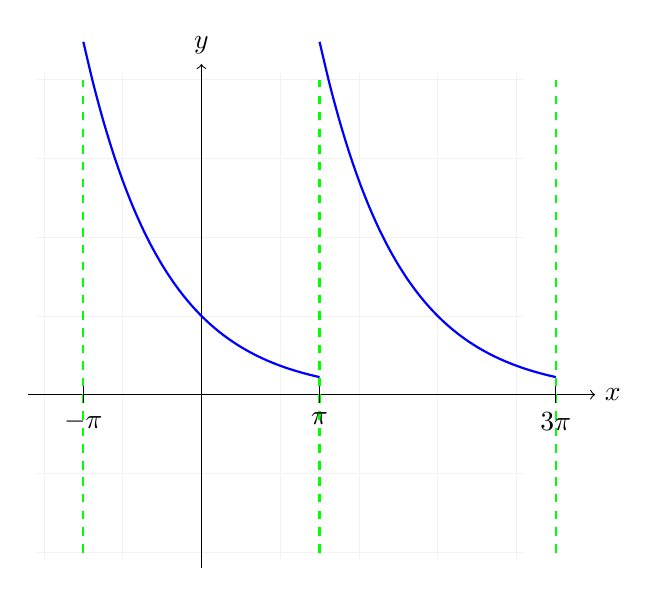
\begin{tikzpicture}
                    \draw[very thin,color=lightgray!20] (-2.1,-2.1) grid (4.1,4.1);
                    \draw[->] (-2.2,0) -- (5,0) node[right] {$x$};
                    \draw[->] (0,-2.2) -- (0,4.2) node[above] {$y$};
                    
                    \draw[thick,green,dashed,domain=-2:4,smooth]plot (-1.5,\x);
                    \draw[thick,green,dashed,domain=-2:4,smooth]plot (1.5,\x);
                    \draw[thick,green,dashed,domain=-2:4,smooth]plot (4.5,\x);

                    \draw[thick,blue,domain=-1.5:1.5,smooth] plot (\x,{exp(-\x)}) node [below right] {};
                    \draw[thick,blue,domain=1.5:4.5,smooth] plot (\x,{exp(-\x+3)}) node [below right] {};

                    \draw[shift={(-1.5,0)},color=black] (0pt,3pt) -- (0pt,-3pt) node[below] {$-\pi$};
                    \draw[shift={(1.5,0)},color=black] (0pt,3pt) -- (0pt,-3pt) node[below] {$\pi$};
                    \draw[shift={(4.5,0)},color=black] (0pt,3pt) -- (0pt,-3pt) node[below] {$3\pi$};
                \end{tikzpicture}
                \item Deret cosinus fourier untuk $0 \leq x\leq\pi$.\\
                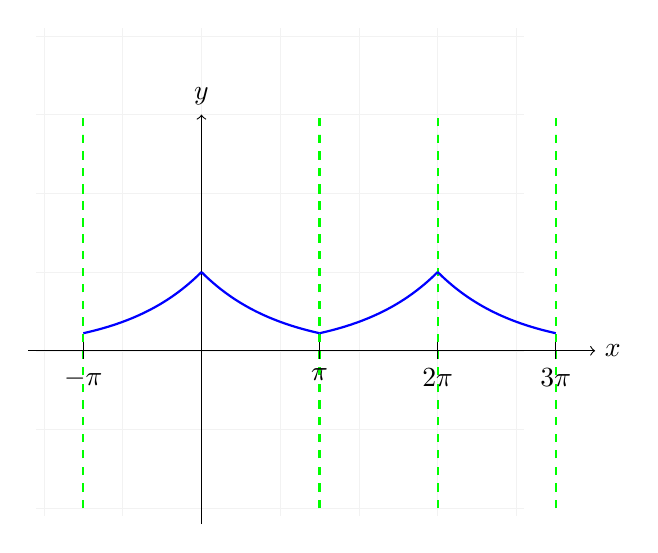
\begin{tikzpicture}
                    \draw[very thin,color=lightgray!20] (-2.1,-2.1) grid (4.1,4.1);
                    \draw[->] (-2.2,0) -- (5,0) node[right] {$x$};
                    \draw[->] (0,-2.2) -- (0,3) node[above] {$y$};
                    
                    \draw[thick,green,dashed,domain=-2:3,smooth]plot (-1.5,\x);
                    \draw[thick,green,dashed,domain=-2:3,smooth]plot (1.5,\x);
                    \draw[thick,green,dashed,domain=-2:3,smooth]plot (3,\x);
                    \draw[thick,green,dashed,domain=-2:3,smooth]plot (4.5,\x);

                    \draw[thick,blue,domain=0:1.5,smooth] plot (\x,{exp(-\x)}) node [below right] {};
                    \draw[thick,blue,domain=-1.5:0,smooth] plot (\x,{exp(\x)}) node [below right] {};
                    \draw[thick,blue,domain=3:4.5,smooth] plot (\x,{exp(-\x+3)}) node [below right] {};
                    \draw[thick,blue,domain=1.5:3,smooth] plot (\x,{exp(\x-3)}) node [below right] {};

                    \draw[shift={(-1.5,0)},color=black] (0pt,3pt) -- (0pt,-3pt) node[below] {$-\pi$};
                    \draw[shift={(1.5,0)},color=black] (0pt,3pt) -- (0pt,-3pt) node[below] {$\pi$};
                    \draw[shift={(3,0)},color=black] (0pt,3pt) -- (0pt,-3pt) node[below] {$2\pi$};
                    \draw[shift={(4.5,0)},color=black] (0pt,3pt) -- (0pt,-3pt) node[below] {$3\pi$};
                \end{tikzpicture}
                \item Deret sinus fourier untuk $0 \leq x\leq\pi$.\\
                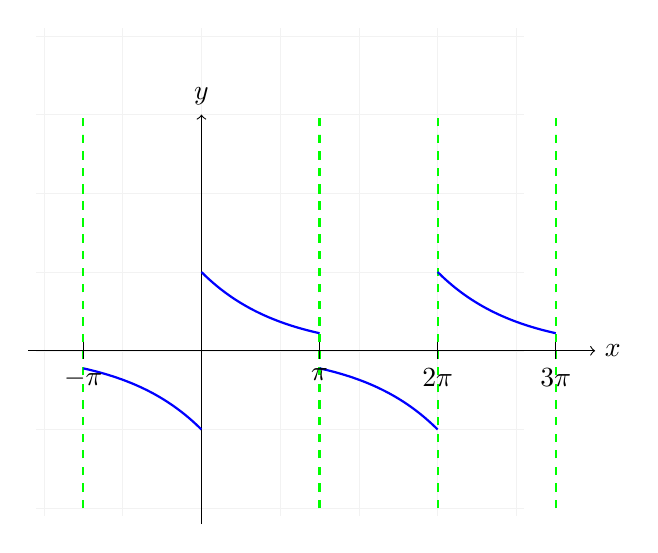
\begin{tikzpicture}
                    \draw[very thin,color=lightgray!20] (-2.1,-2.1) grid (4.1,4.1);
                    \draw[->] (-2.2,0) -- (5,0) node[right] {$x$};
                    \draw[->] (0,-2.2) -- (0,3) node[above] {$y$};
                    
                    \draw[thick,green,dashed,domain=-2:3,smooth]plot (-1.5,\x);
                    \draw[thick,green,dashed,domain=-2:3,smooth]plot (1.5,\x);
                    \draw[thick,green,dashed,domain=-2:3,smooth]plot (3,\x);
                    \draw[thick,green,dashed,domain=-2:3,smooth]plot (4.5,\x);

                    \draw[thick,blue,domain=0:1.5,smooth] plot (\x,{exp(-\x)}) node [below right] {};
                    \draw[thick,blue,domain=-1.5:0,smooth] plot (\x,{-exp(\x)}) node [below right] {};
                    \draw[thick,blue,domain=3:4.5,smooth] plot (\x,{exp(-\x+3)}) node [below right] {};
                    \draw[thick,blue,domain=1.5:3,smooth] plot (\x,{-exp(\x-3)}) node [below right] {};

                    \draw[shift={(-1.5,0)},color=black] (0pt,3pt) -- (0pt,-3pt) node[below] {$-\pi$};
                    \draw[shift={(1.5,0)},color=black] (0pt,3pt) -- (0pt,-3pt) node[below] {$\pi$};
                    \draw[shift={(3,0)},color=black] (0pt,3pt) -- (0pt,-3pt) node[below] {$2\pi$};
                    \draw[shift={(4.5,0)},color=black] (0pt,3pt) -- (0pt,-3pt) node[below] {$3\pi$};
                \end{tikzpicture}
            \end{enumerate}
        \end{enumerate}
    \end{enumerate}
\end{document}
